\documentclass{article}

\usepackage{amsmath, amsthm, amssymb}
\usepackage[round]{natbib}
\usepackage{algorithm}
\usepackage{algpseudocode}
\usepackage[left=2.5cm, right=2.5cm, top=3cm, bottom=3.00cm]{geometry}
\usepackage{array}
\usepackage{booktabs}
\setlength{\heavyrulewidth}{1.5pt}
\setlength{\abovetopsep}{4pt}

% The line below tells R to use knitr on this.
%\VignetteEngine{knitr::knitr}

\title{Elliptical Slice Sampling}
\author{Francesca Panero \and Xuewen Yu}

\usepackage{Sweave}
\begin{document}
\Sconcordance{concordance:my_vignette.tex:my_vignette.Rnw:%
1 14 1 1 0 275 1}


\maketitle

\begin{abstract}
In this project, we present the R package `ESSpackage', which provides an implementation of the elliptical slice sampling method presented by Murray et al. in 2010 $\cite{MAM}$. We validate this algorithm on the simplest scenario of Gaussian regression model with synthetic data, comparing it with the theoretical model and two Metropolis-Hastings algorithms. We tested it on real data, comparing it with one Metropolis-Hastings method.
\end{abstract}

\section{Introduction}

Slice sampling was introduced by Neal in 2003 \cite{Neal2003}. He presented a new approach to sample from a probability density function (called target) from which we are not able to sample, trying to overcome some drawbacks of the two major Markov Chain Monte Carlo (MCMC) methods of sampling: the Gibbs sampler and the Metropolis-Hastings method. The basic idea of MCMC methods is to construct a Markov chain that has as stationary distribution the target one, and samples from this chain will eventually come from the desired distribution.

%Gibbs sampler exploits the possibility of sampling from the full conditional density functions of each parameter given all the others (that are usually simpler to deal with than the original joint distribution), since the complete vector of parameters will eventually be sampled from the joint distribution of these. No tuning of parameters of the chain is required, but we must be able to sample from these conditional distributions in order to implement the method, and sometimes this could not be the case. Nevertheless, some algorithms to overcome this problem have been proposed, in particular ARS (adaptive rejection sampling) and MARS (adaptive rejection Metropolis sampling).
%Metropolis Hasting, instead, initializes the chain with a value sampled from a proposal distribution from which we are able to sample from and that attains some nice links with the target distribution. This sample can be accepted or rejected according to a probability that depends on the likelihood of the new candidate point and the previous one. This method presents some scale parameters for which there does not exist a certain rule of decision; moreover, the proposal distribution does not always come from a straightforward reasoning.

%Slice sampling tries to overcome these flaws in the previous methods.
The simple idea of slice sampling lies in the fact that if we want to sample $x$ from a distribution $p(x)$ that is proportional to a certain function $f(x)$, it is sufficient to sample $x$ uniformly from the area below $f(x)$.
By defining an auxiliary random variable $y$, we exploit Gibbs sampling to sample from the two full conditional distributions of $x$ and $y$. In particular, $y|x$ is distributed as an $Uniform(0,f(x))$ and $x|y$ is distributed as an uniform on the so called slice $S=\lbrace x: y<f(x)\rbrace$. The joint density of $x$ and $y$ is, then $$p(x,y)=\begin{cases}1/Z\quad&\text{ for }0<y<f(x)\\0\quad&\text{ otherwise}\end{cases}$$where $Z=\int f(x)dx$. Of course, $p(x)=\int_0^{f(x)} p(x,y)dy=(1/Z)f(x)$ as desired.
%Sampling on the slice can be difficult, and it is sometimes substituted with some update for $x$ which leaves invariant the uniform distribution.

Based on this idea, Murray et al. \cite{MAM} proposed elliptical slice sampling for models with a multivariate Gaussian prior and indicated the advantage of this new method over MCMC methods in terms of computational complexity and performance of the sampled Markov chains.

\section{Elliptical Slice Sampling}

Elliptical Slice Sampling is an MCMC method that avoids the tuning of parameters, simpler and often faster than other methods to sample from the posterior distribution of models with multivariate Gaussian prior.

Let $\mathbf{f}$ be the vector of latent variables distributed as a Gaussian random variable with zero vector mean and covariance matrix $\Sigma$: $$\mathbf{f}\sim\mathcal{N}(\mathbf{f};\mathbf{0}, \Sigma)=|2\pi\Sigma|^{-1/2}\text{exp}\left(-\frac{1}{2}\mathbf{f}^T\Sigma^{-1}\mathbf{f}\right)$$ Let $$L(\mathbf{f})=p(\text{data}|\mathbf{f})$$ be the likelihood function. Our target distribution is the posterior of this model: $$p^*(\mathbf{f})\propto \mathcal{N}(\mathbf{f};\mathbf{0}, \Sigma)L(\mathbf{f}).$$

The starting point of \cite{MAM} dates back to 1999, when Neal \cite{Neal} introduced the idea of a Metropolis-Hastings algorithm for this type of problems, by proposing a new state of the Markov chain according to
$$\mathbf{f^{'}}=\sqrt{1-\epsilon^2}\mathbf{f}+\epsilon\pmb{\nu},\qquad\pmb{\nu}\sim\mathcal{N}(\mathbf{0}, \Sigma),$$ that represents half of an ellipse as function of $\epsilon\in[-1,1]$ (called step-size parameter) passing through $\mathbf{f}$ and $\pmb{\nu}$. %When $\epsilon=0$ we are resampling the same value.
The probability of accepting the move was defined as $$p(\text{accept})=\text{min}(1,L(\mathbf{f^'})/L(\mathbf{f})),$$ otherwise the next state will still be $\mathbf{f}$. Neal reported that this method was considerably faster, simpler and more general than Gibbs sampling, but $\epsilon$ needed to be tuned for the Markov chain to mix efficiently.

A richer choice of proposals can be easily given by another parametrization of the whole ellipse, so we will sample our new state according to $$\mathbf{f^{'}}=\pmb{\nu}\text{sin}\theta+\mathbf{f}\text{cos}\theta,$$ where $\theta$ is a new step-size parameter.

The core idea of the elliptical slice sample is to avoid the necessity of tuning the step-size parameter by augmenting the prior to make $\theta$ a random variable and sample it with the slice sampling. The proposed augmented model is
\begin{align*}
\pmb{\nu}_0&\sim\mathcal{N}(\mathbf{0},\Sigma)\\
\pmb{\nu}_1&\sim\mathcal{N}(\mathbf{0},\Sigma)\\
\theta&\sim \text{Uniform}[0,2\pi]\\
\mathbf{f^{'}}&=\pmb{\nu}_0\text{sin}\theta+\pmb{\nu}_1\text{cos}\theta
\end{align*}
which assures that the distribution of $\bf{f}$ is always $\mathcal{N}(\mathbf{0},\Sigma)$. The new target distribution is $$p^*(\pmb{\nu}_0,\pmb{\nu}_1,\mathbf{f})\propto\mathcal{N}(\pmb{\nu}_0;\mathbf{0},\Sigma)\mathcal{N}(\pmb{\nu}_1;\mathbf{0},\Sigma)L(\mathbf{f}(\pmb{\nu}_0,\pmb{\nu}_1,\theta))$$
Then, the first proposed and simpler algorithm exploits slice sampling:\\

\begin{algorithm}
\caption{ESS Algorithm}\label{ess}
\hspace*{\algorithmicindent} \textbf{Input}: $\mathbf{f},\,\text{log}L,\,\Sigma$ \\
\hspace*{\algorithmicindent} \textbf{Output}: $\mathbf{f^{'}}$$\sim p^*$
\begin{algorithmic}[1]
  \State Sample from $p(\pmb{\nu}_0,\pmb{\nu}_1,\theta|\pmb{\nu}_0\text{sin}\theta+\pmb{\nu}_1\text{cos}\theta=\mathbf{f})$:
\begin{align*}
\theta &\sim\text{Uniform}[0,2\pi]\\
\pmb{\nu}&\sim\mathcal{N}(\mathbf{0},\Sigma)\\
\pmb{\nu}_0 &\leftarrow\mathbf{f}\text{sin}\theta+\pmb{\nu}\text{cos}\theta\\
\pmb{\nu}_1 &\leftarrow\mathbf{f}\text{cos}\theta-\pmb{\nu}\text{sin}\theta
\end{align*}
  \State Sample $\theta$ using slice sampling on $p^*(\theta|\pmb{\nu}_0,\pmb{\nu}_1)\propto L(\pmb{\nu}_0\text{sin}\theta+\pmb{\nu}_1\text{cos}\theta)$
  \State\textbf{Return} $\mathbf{f^{'}}=\pmb{\nu}_0\text{sin}\theta+\pmb{\nu}_1\text{cos}\theta$
%\EndProcedure
\end{algorithmic}
\end{algorithm}

To avoid proposing $\pmb{\nu}_{0}$ and $\pmb{\nu}_{1}$ in every iteration of the algorithm and to shrink the range of $\theta$ after every iteration in order to avoid rejectios, Murray et al. \cite{MAM} suggested the more mature algorithm \ref{ess*}:

\begin{algorithm}
\caption{Neater ESS Algorithm}\label{ess*}
\hspace*{\algorithmicindent} \textbf{Input}: $\mathbf{f},\,\text{log}L,\,\Sigma$ \\
\hspace*{\algorithmicindent} \textbf{Output}: $\mathbf{f^{'}}$$\sim p^*$
\begin{algorithmic}[1]
\State Sample $\pmb{\nu}\sim\mathcal{N}(\mathbf{0},\Sigma)$ (this defines the ellipse centered in the origine and passing through $\mathbf{f}$ and $\pmb{\nu}$).
%\algstore{<ess>}
%%\end{algorithmic}
%\end{algorithm}

%\begin{algorithm}
%\begin{algorithmic}[1]
%\algrestore{<ess>}
\State Define the slice by sampling the height $y$:
\begin{align*}
u &\sim\text{Uniform}[0,1]\\
\text{log}y &\leftarrow \text{log}L(\mathbf{f})+\text{log}u
\end{align*}
\State Define the bracket for the angles:
\begin{align*}
\theta &\sim\text{Uniform}[0,2\pi]\\
[\theta_{\text{min}},\theta_{\text{max}}]&\leftarrow [\theta-2\pi,\theta]
\end{align*}
\State Propose a new status $\mathbf{f^{'}}\leftarrow\mathbf{f}\text{cos}\theta+\pmb{\nu}\text{sin}\theta$
\If{$\text{log}L(\mathbf{f^{'}})>\text{log}y$}
    \State Accept: \textbf{return} $\mathbf{f^{'}}$
\Else{ Shrink the range of the angles:
    \If{$\theta<0$} $\,\theta_{min}\leftarrow\theta$, \textbf{else} {$\;\theta_{max}\leftarrow\theta$}
    \EndIf
    \State $\theta\sim\text{Uniform}[\theta_{min}, \theta_{max}]$
    \State Go to 4.}
\end{algorithmic}
\end{algorithm}

\begin{figure}
    \centering
    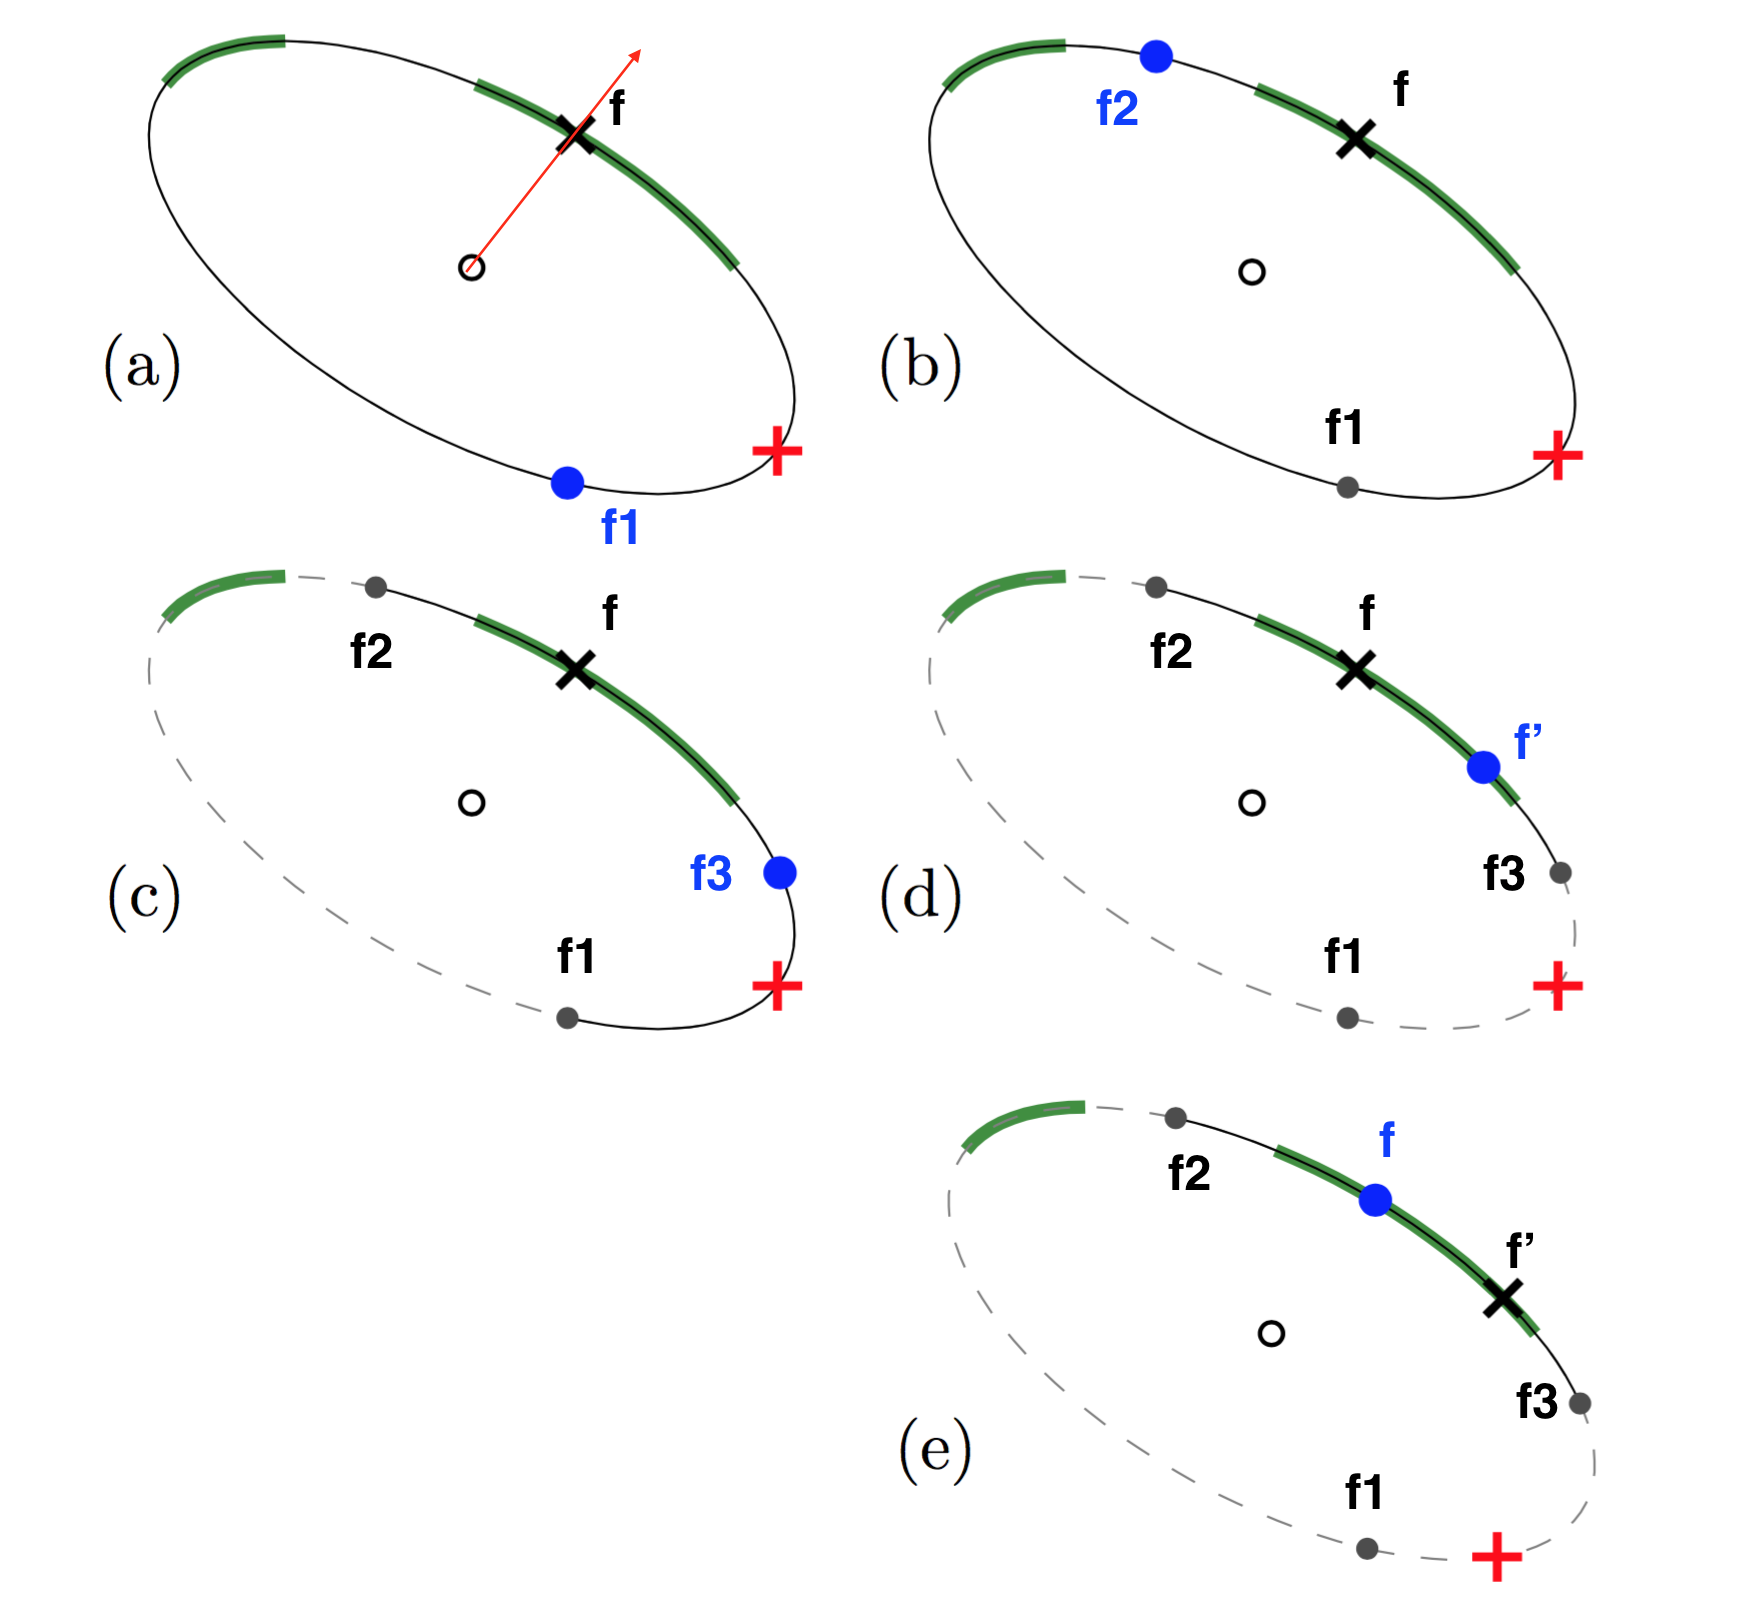
\includegraphics[width = 10cm,height = 8cm]{essfig.png}
    \caption{(a)-(d): The initial state $\bf{f}$ is denoted by the black cross, the red cross represents the auxiliary variable $\pmb{\nu}$, the green slices the likelihood threshold, the blue points are the new proposals in each step and solid lines are the range from which $\theta$s are sampled. (e) is the reverse procedure proposing $\bf{f}$ back from $\bd{f'}$, where $\bf{\nu'}$ is the red cross.}
\end{figure}

An example of updating $\bf{f}$ to $\bf{f'}$ by implementing this algorithm is shown in Figure 1. $\bf{f}$ is the location where $\theta = 0$. The green line highligths the slices defined by step $2$ and in which our new state $\bf{f'}$ must lie to satisfie the constraint in step $5$.The four proposals are $\bf{f_1}, \bf{f_2}, \bf{f_3}$ and $\bf{f_4}$, where $\bf{f_4} = \bf{f'}$, that correspond to angles $\theta_k$ $k=1,...,4$. The range from which $\theta$s are sampled shrinks during the running of the algorithm in a way such that $\bf{f}$ is always included. The update stops when the proposed new state lies on the green slice, i.e. the range of likelihood satisfying step $5$ in the algorithm. This process is reversible and, starting from $\mathbf{f^'}$, the original state $\bf{f}$ can be reached, as shown in $(e)$. When we update the state from $\bf{f'}$, $\theta = 0$ at this point. A rotation of $-\theta_4$ will return back to the original state and rotations of $\theta_i-\theta_4$ bring back to the states $\mathbf{f}_i\;i=1,2,3$.


\section{Experiments}
In this section, we will validate and test the elliptical slice sampling algorithm on two examples, Gaussian regression and Log Gaussian Cox process, and compare this algorithm with other Metropolis-Hastings procedures.

\subsection{Model Description}
\subsubsection{Gaussian Regression}

In this model we have the usual prior parameter $\bf{f}$ $= (f_1,...,f_N)$ that is $\sim{ mathcal{N(\mathbf{0},\Sigma)}}$. Observations $y_n$ are drawn from a Normal distribution with mean $f_n$ and variance $\sigma_n^2$, for $n = 1,...,N$. To simulate $\bf{f}$, we define the covariance matrix as
\begin{equation}\label{covmat}
\Sigma_{i,j} = \sigma_{f}^{2}\text{exp}\left(-\frac{1}{2}\sum_{d=1}^{D}(x_{d,i} - x_{d,j})^2/l^2\right)
\end{equation}
where $\mathbf{x}_n$, $n = 1,...,N$, are the $D$-dimensional input vectors drawn from a $D$-dimensional unit hypercube for all $n$.
Fixing $l$ (called ``lengthscale" parameter), $\sigma_{f}^2$ and $\sigma_{n}^2$, we can generate $\mathbf{f}_n$ and therefore simulate observations $y_n$, since $\mathbf{y}|\mathbf{f}\sim\mathcal{N}\left(\mathbf{f},\sigma_n^2\mathbf{I}\right)$:
\begin{equation}
L_r(\mathbf{f}) = \prod_{n=1}^{N} \mathcal{N}(y_n;f_n,\sigma_n^2)
\end{equation}


\subsubsection{Log Gaussian Cox process}
  Cox process is a "doubly stochastic" Poisson process with a stochastic intensity measure.
  Log Gaussian Cox process is introduced by Moller \cite{Moller}
  as the Cox process where the logarithm of the intensity function is a Gaussian process. Mathematically, let $y_n$ denote the observations. Then $y_n \sim{Poisson(\lambda_n)}$. The intensity function can be estimated given the log Gaussian Cox process observations within a bounded subset. This means we can partition the space finitely into $N$ bins and $y_n$ will represent the number of events in bin $n$ for all $n = 1,...,N$. We assume that every bin has a constant intensity function $\lambda_n$. Let $m$ be the offset to the log mean $\lambda_n$, and define it as the sum of the mean log-intensity of the Poisson process and the log of the bin size.
  \begin{equation}
  y_n|f_n \sim{Poisson(exp(f_n + m))}
  \end{equation}
  \begin{equation}
  \mathbf{f} \sim\mathcal{N}(\mathbf{0},\Sigma)
  \end{equation}

The prior covariance matrix $\Sigma$ is defined as in the Gaussian regression example \ref{covmat}.
%Then, the likelihood of $\bf{y}$ is:
  %\begin{equation}
  %L_p(\bf{f}) = \prod_{n=1}^{N}\frac{\lambda_{n}^{y_{n}} exp(-\lambda_n)}{y_n!}, \lambda_n = e^{f_n+m}
  %\end{equation}

\subsection{Implementation and Results}
\subsubsection{Gaussian Regression}

Let $l=1$, $\sigma_{f}^2 = 1$, $\sigma_{n}^2 = 0.3^2$. Firstly, we validate the elliptical slice sampling algorithm on a Gaussian regression model when $\bf{f}$ is a bivariate normal random variable, hence $N = 2$. We decided to set $D = 1$ so that $x_1,x_2$ are one dimensional. Since both prior distribution and likelihood function are Gaussian, the posterior distribution of $\bf{f}$ will be Gaussian. We perform Henze-Zirkler's test to assess whether the outputs follow a bivariate normal distribution. This is based on the measure of distance, which is nonnegative, between the characteristic function of the multivariate normality and the empirical characteristic function. The distribution of the test statistic is approximately log normal. We achieved a p-value much larger than 0.05, which indicates that there is no strong evidence to reject the null hypothesis that the outputs of the algorithm follow a multivariate normal distribtuion. We can visualise the distribution of outputs in figure \ref{fig1}.
%As a necessary condition for mutivariate normality, each variable should have normal distribution. We confirm this condition from QQ-plot.

\begin{figure} [h!]\label{fig1}
\centering
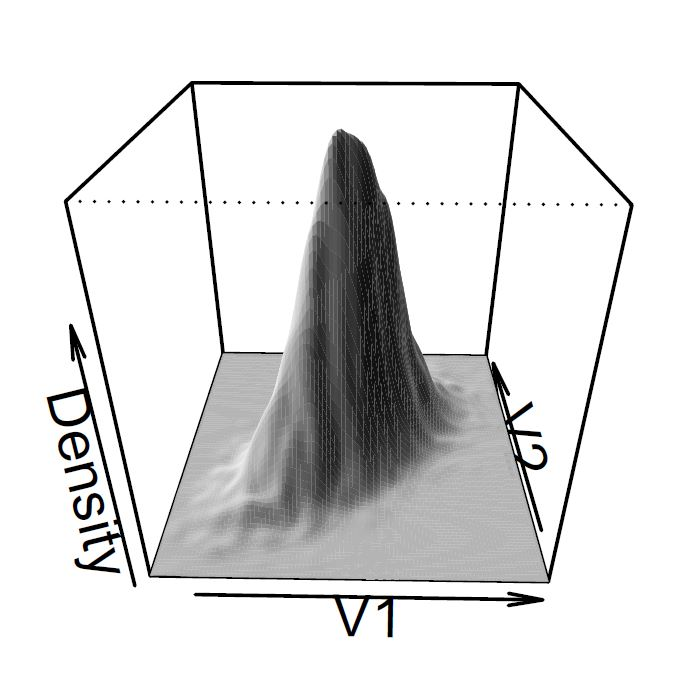
\includegraphics[width=4cm]{3dplot.JPG}
\caption{Perspective plot for bivariate outputs}
\end{figure}
%\begin{figure} [h!]
%\centering
%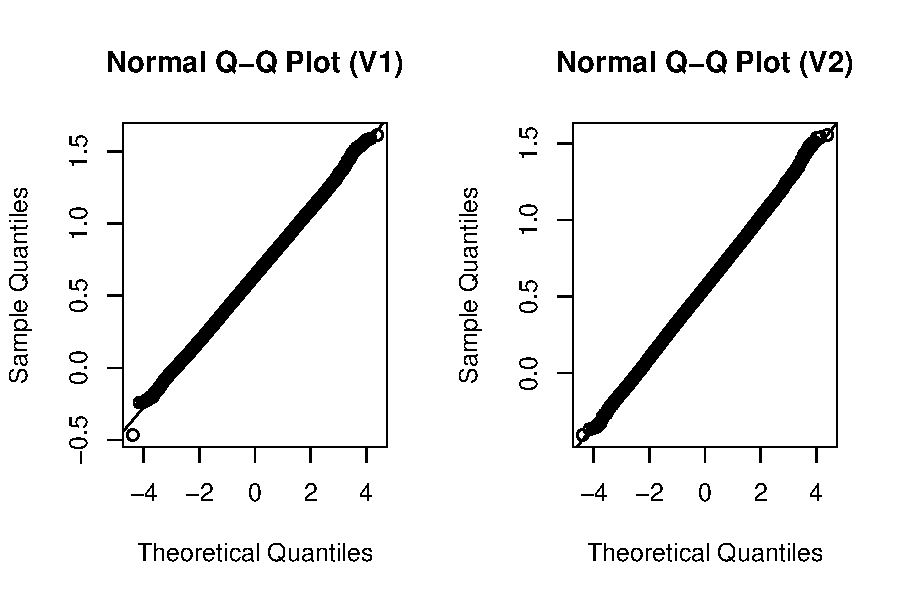
\includegraphics[width = 10cm]{qqplot.pdf}
%\caption{QQ plot of $f_1$ and $f_2$ from Elliptical Slice Sampling algorithm }
%\end{figure}

Then we assess the performance of the algorithm on a Gaussian regression when $N=200$, i.e. $\bf{f}$ is 200-dimensional. As stated in the model description section, $\bf{f}$ can be generated by inputing $\mathbf{x}_n\;n=1,\dots,200$ to covariance matrix. So we first simulated datasets $\mathbf{x}_n\sim\text{Uniform}[0,1]^D$. In order to compare the performance of algorithm for different dimensions of input vectors, i.e. $D$, two synthetic datasets $\lbrace\mathbf{x}^1_n\rbrace_{n=1}^{200}$,$\lbrace\mathbf{x}^{10}_n\rbrace_{n=1}^{200}$ will be simulated with $D = 1,10$ respectively. Denote the observations simulated from these two cases as $R1$ and $R10$ respectively.
%\begin{figure} [h!]
%\centering
%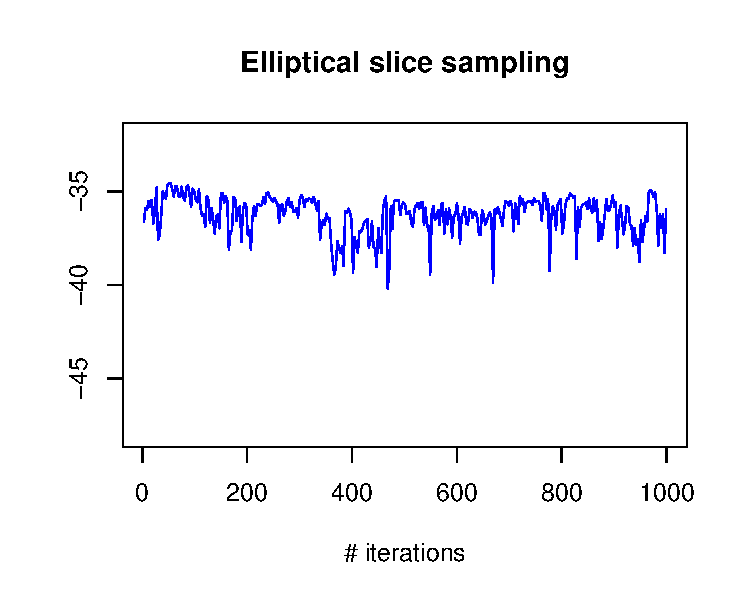
\includegraphics[width = 10cm]{figure1.pdf}
%\caption{Trace plot of log likelihood of 333 points in the first 1000 iterations by taking every 3 iterations}
%\end{figure}
%\begin{figure}[h!]
%\centering
%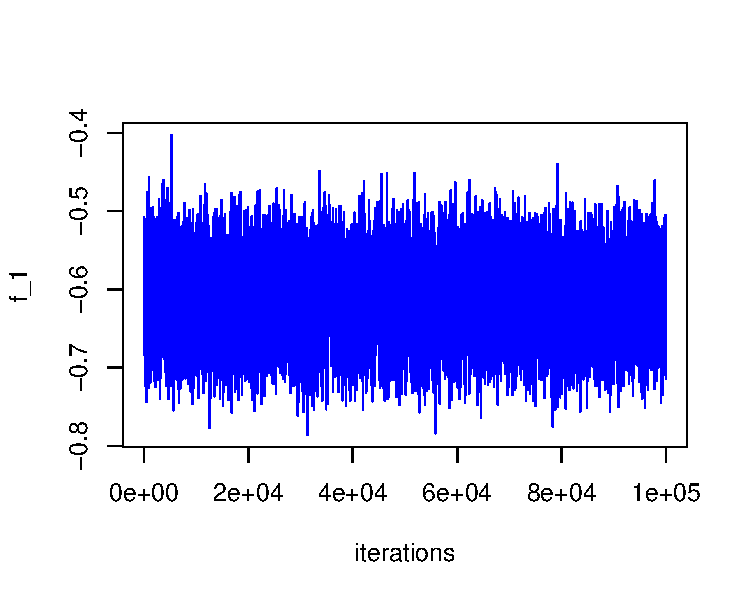
\includegraphics[width = 10cm]{tracef_1.pdf}
%\caption{Trace plot of the first dimension dimension of output $f$ of 100000 iterations}
%\end{figure}
%The traces of log-likelihoods and the first dimension of outputs for $D=1$ are shown in Figure 3 and 4 respectively, which reveal frequent jumps in both chains. The effective sample size for it is 3177.

\subsubsection{Log Gaussian Cox process}

Data of mining disasters are provided by Jarrett et al. \cite{Jarrett}. There were 191 events happening during 40550 days which were partitioned into 811 bins each containing 50 days, according to Murray et al. $\cite{MAM}$. $\mathbf{f}$, therefore, is 811 dimensional and this considerably affects the running time of both elliptical slice samping and Metropolis-Hastings. Hence, we decided to partition the period into 102 bins, such that each interval includes 400 days (except the last one, which consists of 150 days). Given the date of every event, the number of events occurred in each bin can be computed, i.e. $y_n$. Accordingly to Murray et al., we set $l=13516$, $\sigma_f^2 = 1$, $N = 102$, $D=1$ and $m=log(191/102)$. We observed frequent jumps in the trace plot of the samples and the autocorrelation function going to 0 after 10 lags.
%\begin{figure}[h!]
%\centering
%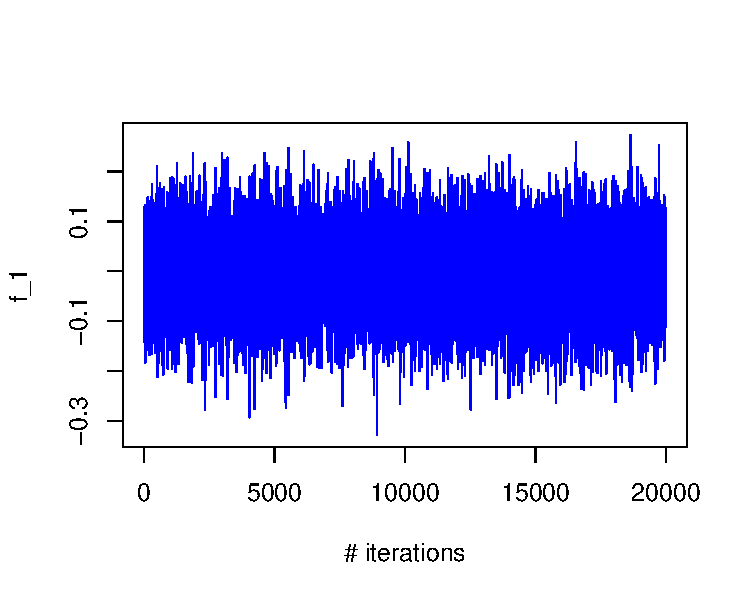
\includegraphics[width = 10cm]{figureminedata.pdf}
%\caption{Trace plot of the first dimension dimension of output $f$ of 20000 iterations}
%\end{figure}

\subsubsection{Comparison}
For Gaussian regression model, we will compare the performance of elliptical slice sampling algorithm with the theorethical Bayesian model, the Metropolis-Hasting algorithm introduced by Neal in \cite{Neal} (the first algorithm described in section 2) and an adapted Metropolis-Hastings algorithm proposed by Roberts et al. in \cite{Roberts}.

In order to plot and compare the densities, we restricted the full $4$-models comparison on the $2$-dimensional case. Hence, $N=2$, $D=1$ and, as suggested in \cite{MAM}, we put $\sigma_n=0.3$, $\sigma_f=1$ and $l=1$.
The full Bayesian model will look like this:
\begin{align*}
\mathbf{f}&\sim \mathcal{N}\left(\mathbf{0},\Sigma\right)\\
\mathbf{y}|\mathbf{f}&\sim\mathcal{N}\left(\mathbf{f},\Sigma^{'}\right)\\
\mathbf{f^'}&\sim\mathcal{N}\left(\left(\Sigma^{-1}+\Sigma^{'}^{-1}\right)^{-1}\Sigma^{'}^{-1}\mathbf{y},\left(\Sigma^{-1}+\Sigma^{'-1}\right)^{-1}\right)
\end{align*}
where $\Sigma$, as proposed before, is such that $\Sigma_{i,j}=\text{exp}\left(-\frac{1}{2}\sum_{d=1}^{2}(x_{d,i} - x_{d,j})^2\right)\,i,j=1,2$ and $\Sigma^{'}=\begin{bmatrix}0.09 & 0 \\ 0 & 0.09\end{bmatrix}$.
We tested the normality of these samples with the `mvnorm.skew.test` from the `ICS` pckage and the null hypothesis was not rejected.

For Neal's Metropolis-Hastings algorithm, we discovered that the performance of the MCMC chain is sensitive to the value of step-size $\epsilon$ because the mixture and convergence of the chain depend on it. We take $\epsilon = 0.2$ after trials of different values.

With the same target distribution, adaptive Metropolis-Hastings (proposed in \cite{Gareth}) uses proposals for the $n^{th}$ iteration as follows:\\
\begin{equation}\label{proposal}
    q_n(\mathbf{f},\mathbf{f'}) =
    \begin{cases}
     \mathcal{N}(\mathbf{f},0.1^2\mathcal{I}_d/d) & n\leq 2d \\
        (1-\beta)\mathcal{N}(\mathbf{f},2.38^2\Sigma_n/d) + \beta \mathcal{N}(\mathbf{f},(0.1^2)\mathbf{I}_d/d) & n > 2d \\
    \end{cases}
\end{equation}

where $\Sigma_n$ is the empirical estimate of the covariance of the target distribution based on the run so far and $\beta$ is a small positive constant.

Compared to other algorithms, adaptive Metropolis-Hastings (MH) algorithm takes longer time to reach a stationary variance and a good mixture. To avoid the complexity derived from the estimation of $\Sigma_n$, in this example, we simply take the covariance of the posterior distribution, which is known. In this case, it is not nessary to take the weighted sum as proposal, which will turn out to be simply $$\mathcal{N}\left(\mathbf{f},2.38^2\left(\Sigma^{-1}+\Sigma^{'-1}\right)^{-1}/d\right)$$.

In the figure \ref{comparison} we can compare the contour plots of the four samples coming from the theoretical model (in green), the ESS algorithm (in blue), the Neal MH (in red) and the adaptive MH (in purple). The number of samples for each model was $100000$, apart from the adaptive MH that needed $500000$ iterations to converge. It is evident that the stationary distributions of the three algorithms are the correct one.
\begin{figure}[H]\label{comparison}
\centering
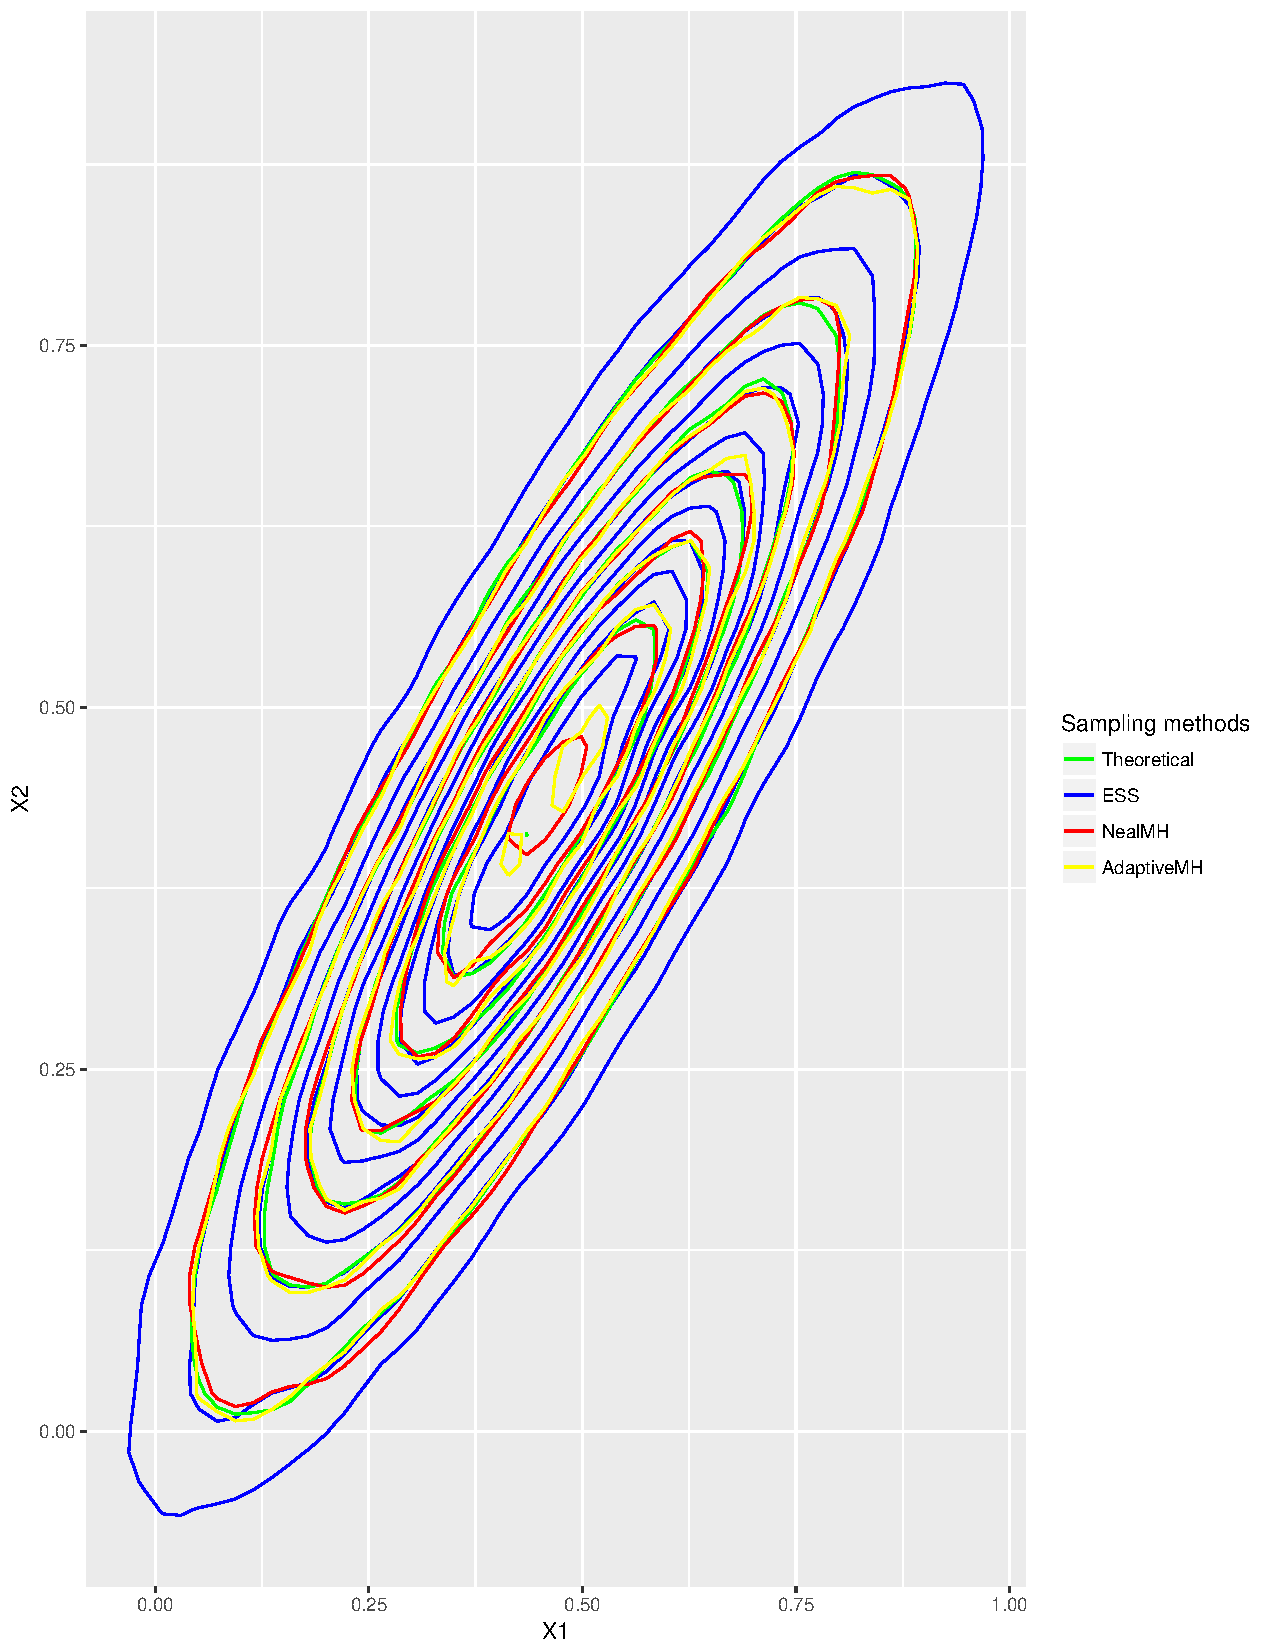
\includegraphics[height=9cm,width = 9cm]{ComparisonGauss.pdf}
\caption{Comparison of contour plots for Gaussian regression: in green theoretical model, in blue ESS, in red Neal MH, in purple adaptive MH}
\end{figure}
%We need to mention the fact that the we tried different step-size parameters for Neal's algorithm to obtain a Gaussian sample. (mentioned)
\vskip 5mm
Then we compared elliptical slice sampling with Neal's MH in terms of effective sample size and CPU time. We run $10^6$ iterations and remove the first $10^5$ as burn-in. We encountered problems when implementing adaptive MH with proposal as shown in equation \ref{proposal}, since we couldn't generate proposals with a positive mass and the chain remained in the same state. Therefore, we only compared elliptical slice sampling with Neal's MH. The results are shown in Table 1, which displays that elliptical slice sampling is more efficient compared to Neal's MH because the former one has more effective samples in all three examples. For mine data, the effective samples were approximately 47\% of the total number of samples for elliptical slice sampling method while consisted of only 21\% of total samples for Neal's MH. For Gaussian regression, on the one hand, the effective sample size is much smaller compared to mine data for both methods, when $\bf{f}$ is 200 dimensional and input vectors are 10 dimensional. On the other hand, the elliptical slice sampling features a longer running time than Neal's MH.

Taking as a measure of efficiency the effective samples per unit time (identified as ``efficiency" in the table), elliptical slice sampling usually outperforms Neal's MH. For example, for $R1$, the effective samples per unit time is 2.1 for elliptical slice sampling, which is approximately twice as large as Neal's MH one.

%\begin{table}[!htbp]
%\centering

%\begin{tabular}{*9c}
%\toprule
% {} &  \multicolumn{3}{c}{R1} & \multicolumn{3}{c}{R10} & \multicolumn{3}{c}{Mining}\\
%\midrule
%\begin{minipage}{\linewidth}
\begin{table}[h]
\begin{center}
\begin{tabular} { c | c c | c c | c c }
{}   & ESS   & NMH    & ESS   & NMH  & ESS   & NMH\\
\hline
effective samples   &  33316.79 & 13330.98   & 2139.793  & 1159.535 & 429181.7 & 186571\\
CPU time   &  15898.001 & 9472.684   & 16374.79  & 10497.30 & 3448.755 & 3271.421\\
efficiency & 2.096 & 1.407 & 0.131 & 0.110 & 124.445 & 57.031 \\
%\bottomrule
\end{tabular}
%\bigskip
\caption{Compare Elliptical Slice Sampling with Neal's Metropolis Hastings on data $R1$, $R10$ and $Mining$ in terms of effective sample size and CPU time.}
%\end{minipage}
%\end{table}
\end{center}
\end{table}


\section{Discussion and Conclusion}

The first advantage we noticed of elliptical slice sampling is that we could avoid parameters to be tuned. When we compared it with Neal's MH, we started using $\epsilon=0.05$ but this parameter didn't mix efficiently, so we tried different ones to get the desired result. It could be useful to find a method to automatically search over the step-size parameter during the running of the algorithm, since every other procedure that proposes different $\epsilon$ outside the main running would be more time consuming.

Regarding the time complexity of elliptical slice sampling, we cannot compare it exactly with Neal's MH since we missed the part of tuning the step-size parameter, but from our results and the ones in the paper \cite{MAM} it seems to be slower than Neal's MH when $\epsilon$ is fixed. For mine data, the running time is more similar, in accordance with the results shown in the paper \cite{MAM}. The same happens for 2 dimensional Gaussian regression.
This slower behavior can be addressed to the lack of a tuning parameter that could reduce the number of likelihood evaluations and speed up the algorithm around two times. Murray et al. highlights that it was their subjective decision not to use a step-size parameter because they found more valuable the absence of it, and therefore the simplicity of implementation, than the doubled running time.

Comparing the efficiency of elliptical slice sampling and Neal's MH, we found that the effective number of samples over the running time is better for our algorithm, although at the cost of higher running time.

To sum up, elliptical slice sampling represents a valid method for sampling from the posterior of models with multivariate Gaussian prior, simple to implement and that performs similarly to Metropolis-Hastings methods.

\begin{thebibliography}{12}

\bibitem{Gareth}
  Gareth O. Roberts & Jeffrey S. Rosenthal (2009)
  \emph{Examples of Adaptive MCMC}, Journal of COmputational and Graphical Statistics, 18:2, 349-367, DOI:10.1198/icgs.2009.06134.

\bibitem{Jarrett}
	Jarrett, R. G.  (1979)
	\emph{A note on the intervals between coal-mining disasters},
	Biometrika.

\bibitem{Moller}
	M{\o}ller, J., Syversveen, A. R., Waagepetersen  (1998)
	\emph{Log Gaussian Cox processes},
	Scandinavian Journal of Statistics.

\bibitem{MAM}
	Murray, I., Adams, R. P., and MacKay, D. J. C. (2010)
	\emph{Elliptical slice sampling},
	Journal of Machine Learning Research.

\bibitem{Neal}
	Neal, R. M. (1999)
	\emph{Regression and Classification Using
Gaussian Process Priors},
	Bayesian Statistics 6 (475-501), OU Press.

\bibitem{Neal2003}
	Neal, R. M. (2003)
	\emph{Slice sampling},
	Annals of Statistics.

\bibitem{Roberts}
	Roberts, G. O., Rosenthal, J. S. (2009)
	\emph{Examples of Adaptive MCMC},
	Journal of Computational and Graphical Statistics.



\end{thebibliography}

\end{document}








